\hypertarget{inits_8c}{
\section{inits.c File Reference}
\label{inits_8c}\index{inits.c@{inits.c}}
}
Some init functions. 

{\tt \#include \char`\"{}smarties2.h\char`\"{}}\par
{\tt \#include \char`\"{}lcd\_\-display.h\char`\"{}}\par
{\tt \#include \char`\"{}inits.h\char`\"{}}\par
{\tt \#include \char`\"{}system.h\char`\"{}}\par
{\tt \#include \char`\"{}menu.h\char`\"{}}\par
{\tt \#include \char`\"{}ee.h\char`\"{}}\par


Include dependency graph for inits.c:\nopagebreak
\begin{figure}[H]
\begin{center}
\leavevmode
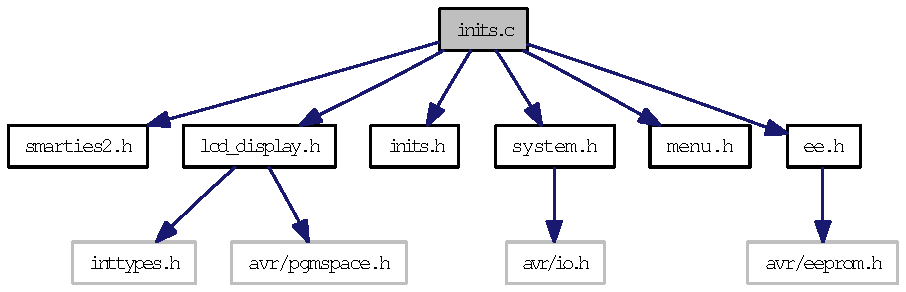
\includegraphics[width=235pt]{inits_8c__incl}
\end{center}
\end{figure}
\subsection*{Functions}
\begin{CompactItemize}
\item 
\hypertarget{inits_8c_c2a3b2c7f1e4975e9080f9f4df57fb84}{
void \hyperlink{inits_8c_c2a3b2c7f1e4975e9080f9f4df57fb84}{init\_\-all} ()}
\label{inits_8c_c2a3b2c7f1e4975e9080f9f4df57fb84}

\begin{CompactList}\small\item\em Calls all necessary init functions. \item\end{CompactList}\item 
\hypertarget{inits_8c_cb9582fdd64e7e2626971cd01ac1a11e}{
void \hyperlink{inits_8c_cb9582fdd64e7e2626971cd01ac1a11e}{init\_\-io} ()}
\label{inits_8c_cb9582fdd64e7e2626971cd01ac1a11e}

\begin{CompactList}\small\item\em Configures nearly all General IO pins, disables JTAG. \item\end{CompactList}\item 
\hypertarget{inits_8c_609556329ca6e7349dd6a4343ebb4218}{
void \hyperlink{inits_8c_609556329ca6e7349dd6a4343ebb4218}{init\_\-sensor\_\-tcs} ()}
\label{inits_8c_609556329ca6e7349dd6a4343ebb4218}

\begin{CompactList}\small\item\em Set up the TCS color sensor. \item\end{CompactList}\item 
void \hyperlink{inits_8c_38016ab7b2931bcb950e0c6f3ba3f342}{init\_\-timer} ()
\begin{CompactList}\small\item\em This will generate an Interrupt every millisecond by Timer 0 on compare match. \item\end{CompactList}\item 
\hypertarget{inits_8c_d0bbdbb6c098b4227028e3f2a0f13770}{
void \hyperlink{inits_8c_d0bbdbb6c098b4227028e3f2a0f13770}{init\_\-memory} ()}
\label{inits_8c_d0bbdbb6c098b4227028e3f2a0f13770}

\begin{CompactList}\small\item\em Inits important system variables, also from EEprom. \item\end{CompactList}\item 
\hypertarget{inits_8c_9907891a049d7bb046be768dfc7717e8}{
void \hyperlink{inits_8c_9907891a049d7bb046be768dfc7717e8}{init\_\-motors} ()}
\label{inits_8c_9907891a049d7bb046be768dfc7717e8}

\begin{CompactList}\small\item\em Brings revolver and catcher to defined positions; Set up important motor values. \item\end{CompactList}\item 
void \hyperlink{inits_8c_5cf20cf8f8b8d7c2aeaaea014d157583}{init\_\-menu} ()
\begin{CompactList}\small\item\em Creates the menu stucture, connects menus, connects functions to menus. \item\end{CompactList}\end{CompactItemize}


\subsection{Detailed Description}
Some init functions. 

Copyright (c) 2008 Simeon Felis 

Definition in file \hyperlink{inits_8c-source}{inits.c}.

\subsection{Function Documentation}
\hypertarget{inits_8c_5cf20cf8f8b8d7c2aeaaea014d157583}{
\index{inits.c@{inits.c}!init\_\-menu@{init\_\-menu}}
\index{init\_\-menu@{init\_\-menu}!inits.c@{inits.c}}
\subsubsection{\setlength{\rightskip}{0pt plus 5cm}void init\_\-menu ()}}
\label{inits_8c_5cf20cf8f8b8d7c2aeaaea014d157583}


Creates the menu stucture, connects menus, connects functions to menus. 

The menu structure and functionality is explained in \hyperlink{menu_8h}{menu.h} in detailed. 

Definition at line 228 of file inits.c.

References menu\_\-entry\_\-t::function, menu\_\-entry\_\-t::l\_\-action, menu\_\-entry\_\-t::next, menu\_\-entry\_\-t::prev, menu\_\-entry\_\-t::r\_\-action, menu\_\-entry\_\-t::submenu, sys\_\-catcher\_\-rotate(), sys\_\-enter\_\-submenu(), sys\_\-enter\_\-topmenu(), sys\_\-measure\_\-tcs(), sys\_\-pause(), sys\_\-reference\_\-measure\_\-blue(), sys\_\-reference\_\-measure\_\-brown(), sys\_\-reference\_\-measure\_\-green(), sys\_\-reference\_\-measure\_\-orange(), sys\_\-reference\_\-measure\_\-pink(), sys\_\-reference\_\-measure\_\-purple(), sys\_\-reference\_\-measure\_\-red(), sys\_\-reference\_\-measure\_\-restore(), sys\_\-reference\_\-measure\_\-yellow(), sys\_\-resume(), sys\_\-revolver\_\-rotate(), sys\_\-speed\_\-down(), sys\_\-speed\_\-up(), menu\_\-entry\_\-t::text, and menu\_\-entry\_\-t::topmenu.

Referenced by init\_\-all().\hypertarget{inits_8c_38016ab7b2931bcb950e0c6f3ba3f342}{
\index{inits.c@{inits.c}!init\_\-timer@{init\_\-timer}}
\index{init\_\-timer@{init\_\-timer}!inits.c@{inits.c}}
\subsubsection{\setlength{\rightskip}{0pt plus 5cm}void init\_\-timer ()}}
\label{inits_8c_38016ab7b2931bcb950e0c6f3ba3f342}


This will generate an Interrupt every millisecond by Timer 0 on compare match. 

The interrupt settings are related like following: \[ T_{Compare Match} = (F_{CPU})^{-1} \cdot Prescaler \cdot (Register_{OutputCompare}) \]

There is an error of about 0.8\% from 1 Millisecond 

Definition at line 123 of file inits.c.

Referenced by init\_\-all().